% appendix of extras

\chapter{延伸内容}

\section{力学延伸}

\subsection{平抛运动抛物线验证}

\begin{equation*}
    \begin{cases}
        x=v_0t\\
        y=\frac12gt^2
    \end{cases}\implies
    y=\frac{g}{2{v_0}^2}x^2
\end{equation*}

\subsection{动能推导}

\begin{equation*}
    E_k=\int\vec{F}\cdot d\vec{s}
        =\int m\vec{a}\cdot d\vec{s}
        =\int m\vec{v}\cdot d\vec{v}
        =\frac12mv^2
\end{equation*}

\subsection{机械能守恒推导}

\begin{align*}
    \int_{t_1}^{t_2}mv\frac{dv}{dt}dt&=\int_{t_1}^{t_2}F\frac{dx}{dt}dt\\
    m\int_{v_1}^{v_2}vdv&=\int_{x_1}^{x_2}Fdx\\
    m\int_{v_1}^{v_2}vdv&=\int_{x_0}^{x_2}Fdx-\int_{x_0}^{x_1}Fdx\\
    \Delta E_k&=-\Delta U\\
    \Delta E_k+\Delta U&=0
\end{align*}

\subsection{重力势能推导}

\begin{equation*}
    E_p=W=\int_{-h}^0mg\cdot dx=mgh
\end{equation*}

\subsection{弹力势能推导}

\begin{equation*}
    E_p=W=\int_{x}^0-k\Delta x\cdot d\Delta x=\frac12kx^2
\end{equation*}

\subsection{动量与冲量关系推导}

\begin{equation*}
    \int_{t_1}^{t_2}Fdt
    =\int_{t_1}^{t_2}m\frac{dv}{dt}dt
    =\int_{v_1}^{v_2}mdv
    =mv_2-mv_1
\end{equation*}

\subsection{圆周运动向心加速度推导}

\begin{gather*}
    v=\left(\frac{dx}{dt},\frac{dy}{dt}\right)
    =(-r\omega\sin\omega t,r\omega\cos\omega t)\\
    a=\left(\frac{dv_x}{dt},\frac{dv_y}{dt}\right)
    =(-r\omega^2\cos\omega t,-r\omega^2\sin\omega t)
    =-\omega^2\vec{r}
\end{gather*}

\subsection{单摆周期推导}

\begin{equation*}
    F\approx -mg\sin\theta=-mg\cdot\frac{x}{l}=-\frac{mg}{l}x
\end{equation*}

\subsection{开普勒定律推导}

将直角坐标系转换为极坐标系处理,
\begin{equation*}
    \begin{pmatrix}
        A_r\\ A_\phi
    \end{pmatrix}=
    \begin{pmatrix}
        \cos\phi & \sin\phi\\
        -\sin\phi & \cos\phi
    \end{pmatrix}
    \begin{pmatrix}
        A_x\\ A_y
    \end{pmatrix}
\end{equation*}
由关系式$x=r\cos\phi,y=r\sin\phi$重复计算可得,$r$方向和$\phi$方向的速度为:
\begin{gather*}
    v_x=\dot{x}=\dot{r}\cos\phi-r\dot{\phi}\sin\phi\\
    v_y=\dot{y}=\dot{r}\sin\phi+r\dot{\phi}\cos\phi\\
    \Downarrow\\
    v_r=v_x\cos\phi+v_y\sin\phi=\dot{r}\\
    v_\phi=-v_x\sin\phi+v_y\cos\phi=r\dot{\phi}
\end{gather*}
$r$方向和$\phi$方向的加速度为:
\begin{gather*}
    a_x=\ddot{x}=(\ddot{r}-r\dot{\phi}^2)\cos\phi-(2\dot{r}\dot{\phi}+r\ddot{\phi})\sin\phi\\
    a_y=\ddot{y}=(\ddot{r}-r\dot{\phi}^2)\sin\phi+(2\dot{r}\dot{\phi}+r\ddot{\phi})\cos\phi\\
    \Downarrow\\
    a_r=a_x\cos\phi+a_y\sin\phi=\ddot{r}-r\dot{\phi}^2\\
    a_\phi=-a_x\sin\phi+a_y\cos\phi=2\dot{r}\dot{\phi}+r\ddot{\phi}=\frac1r\frac{d}{dt}(r^2\dot{\phi})
\end{gather*}
如此一来行星的$r$方向和$\phi$方向的运动方程即为
\begin{gather*}
    m(\ddot{r}-r\dot{\phi}^2)=-G\frac{Mm}{r^2}\\
    m\frac1r\frac{d}{dt}(r^2\dot{\phi})=0
\end{gather*}
由$\phi$方向的运动方程可知$r^2\dot{\phi}$为与时间无关的常数,其形式可以用扇形面积公式的方式解释为面积速度。因此$r^2\dot{\phi}=h$,开普勒第二定律得证。

随后用$\dot{\phi}=\frac{h}{r^2}$改写$r$方向的运动方程可得
\begin{equation*}
    \ddot{r}-\frac{h^2}{r^3}=-\frac{GM}{r^2}
\end{equation*}
其中
\begin{gather*}
    \dot{r}=\frac{dr}{dt}=\frac{dr}{d\phi}\frac{d\phi}{dt}=\frac{h}{r^2}\frac{dr}{d\phi}\\
    \ddot{r}=\frac{d\dot{r}}{d\phi}\frac{d\phi}{dt}=\frac{h}{r^2}\left(\frac{d}{d\phi}\left(\frac{h}{r^2}\frac{dr}{d\phi}\right)\right)
\end{gather*}
代入上式可得
\begin{equation*}
    \frac{d}{d\phi}\left(\frac{1}{r^2}\frac{dr}{d\phi}\right)-\frac1r=\frac{-GM}{h^2}
\end{equation*}
在此将$\frac1r$置换为$u$,即$dr=\frac{-1}{u^2}du$,则有
\begin{align*}
    \frac{d}{d\phi}\left(u^2\frac{-1}{u^2}\frac{du}{d\phi}\right)-u&=\frac{-GM}{h^2}\\
    \frac{d}{d\phi}\frac{du}{d\phi}+u&=\frac{GM}{h^2}\\
    \frac{d^2u}{d\phi^2}+u&=\frac1l
\end{align*}
求解非齐次常微分方程可得
\begin{equation*}
    u=A\cos(\phi+\phi_0)+\frac1l
\end{equation*}
取$\phi_0=0$,设$A=\frac{\varepsilon}{l}$,整理可得
\begin{equation*}
    r=\frac{l}{\varepsilon\cos\phi+1}
\end{equation*}
即行星轨道为圆锥曲线,具体形状取决于其离心率。开普勒第一定律得证。

最后,由椭圆面积公式可求行星公转周期为
\begin{equation*}
    T=\frac{\pi ab}{h/2}
\end{equation*}
结合$l$的数学意义(半正焦弦:$al=b^2$)和物理意义($\frac1l=\frac{GM}{h^2}$)可得
\begin{equation*}
    T^2=\frac{4\pi^2 a^2b^2}{h^2}
    =\frac{4\pi^2la^3}{h^2}
    =\frac{4\pi^2}{GM}a^3
\end{equation*}
至此开普勒第三定律得证。

\subsection{万有引力势能推导}

\begin{equation*}
    E_p=W=\int_r^\infty-G\frac{Mm}{x^2}dx=-G\frac{Mm}{r}
\end{equation*}

\section{热学延伸}

\subsection{理想气体内能公式推导}

如图,气体分子在边长为l的立方体容器内运动、三个方向上的速度均为$v$,假设其与容器壁做弹性碰撞,计算气体压强与分子运动速度的关系。
\begin{figure}[ht!]
    \centering
    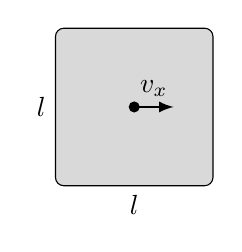
\begin{tikzpicture}
        \filldraw[color=black, fill=gray!30, rounded corners=3pt] (0, 0) rectangle (2, 2);
        \node[below] at (1, 0) {$l$};
        \node[left] at (0, 1) {$l$};
        \draw[thick, -latex] (1, 1) -- node[above] {$v_x$} ++ (0.5, 0) ;
        \fill (1, 1) circle (2pt);
    \end{tikzpicture}
    \caption{气体分子运动与压强}
\end{figure}
由于气体分子在x方向上每折返一次就会与容器壁发生一次碰撞,所以$\Delta t$时间内会与容器壁碰撞$\frac{v\Delta t}{2l}$次。因此这段时间内容器壁受到来自气体分子的冲量为
\begin{equation*}
    2mv\cdot\frac{v_x\Delta t}{2l}=\frac{m{v_x}^2}{l}\Delta t
\end{equation*}
即相当于单个气体分子给予容器壁$F=\frac{m{v_x}^2}{l}$大小的力,相对应的就会有
\begin{equation*}
    P=\frac{F}{l^2}=\frac{m{v_x}^2}{l^3}=\frac{m{v_x}^2}{V}
\end{equation*}
大小的压强。此外,该气体分子也会在y和z方向上做同样的运动,所以其速度的平均值为$\overline{v^2}=\overline{{v_x}^2}+\overline{{v_y}^2}+\overline{{v_z}^2}$。同时,容器内倘若有N个这样的气体分子,那么其压强的总和为
\begin{equation*}
    P=N\cdot\frac{m{v_x}^2}{V}=\frac{Nm\overline{v^2}}{3V}
\end{equation*}
将上述压强值代入理想气体状态方程就可以得到1摩尔该气体分子平均速度的平方。
\begin{gather*}
    PV=nRT\\
    \frac{Nm\overline{v^2}}{3V}V=\frac{N}{N_A}RT\\
    \overline{v^2}=\frac{3RT}{M}
\end{gather*}
那么n摩尔该气体分子的总动能可求。
\begin{equation*}
    n\cdot\frac12M\overline{v^2}=\frac32nRT
\end{equation*}

\subsection{等温变化做功}

\begin{equation*}
    Q_\textrm{吸}=W_\textrm{した}=\int_{V_1}^{V_2}PdV=nRT\cdot\log\frac{V_2}{V_1}
\end{equation*}

\subsection{断热变化PV等式推导}

基于断热变化的热力学第一定律可得
\begin{gather*}
    \Delta U=-W_\textrm{した}\\
    nC_v\Delta T=-PdV
\end{gather*}
简做整理后对两侧分别关于T和V积分
\begin{gather*}
    \int\frac{dT}{T}=-\frac{R}{C_v}\int\frac{dV}{V}\\
    \log T=-\frac{R}{C_v}\log V+c^\prime\\
    T=V^{-\frac{R}{C_v}}\cdot c\\
    TV^{\frac{R}{C_v}}=c
\end{gather*}
在此定义$\gamma=\frac{C_p}{C_v}$,结合$C_p-C_v=R$即有
\begin{equation*}
    TV^{\gamma-1}=c
\end{equation*}
再结合理想气体状态方程就可以得到$PV^\gamma=const$的结论。

\section{波动延伸}

\subsection{波的解析式推导法二}

假设$t=0$时刻的波形为
\begin{equation*}
    y_0=A\sin\left(\frac{2\pi}{\lambda}x\right)
\end{equation*}
那么$t$时间后改图像会向右平移$vt$单位长度,即
\begin{equation*}
    y=A\sin\left(\frac{2\pi}{\lambda}\left(x-vt\right)\right)
    =A\sin\left(2\pi\left(\frac{x}{\lambda}-\frac{t}{T}\right)\right)
\end{equation*}

\subsection{差频公式推导}

设两束声波分别为$y_1=\sin((\omega+\theta)t)$和$y_2=\sin((\omega-\theta)t)$,其中$\omega$远大于$\theta$。那么,根据波的叠加原理可知合成波为
\begin{align*}
    y=&\sin((\omega+\theta)t)+\sin((\omega-\theta)t)\\
    =&(\sin\omega t\cos\theta t+\cos\omega t\sin\theta t)+(\sin\omega t\cos\theta t-\cos\omega t\sin\theta t)\\
    =&(2\cos\theta t)\sin\omega t
\end{align*}
此外,声音的强度与振幅的平方相关,所以合成波的波峰与波谷都会被人耳当成差频接收。因此差频的频率为合成波括号中控制振幅部分频率的两倍。
\begin{align*}
    f=&2\times\frac{\theta}{2\pi}\\
    =&\frac{\omega_1-\omega_2}{2\pi}\\
    =&f_1-f_2
\end{align*}

\subsection{光程公式推导}

使波长为$\lambda$的波在折射率为$n$的介质中传播$l$长的距离,那么在这段空间中存在$\frac{l}{\lambda^\prime}=\frac{nl}{\lambda}$个波。倘若把这些波换算到真空中($n=1$)中,则需要
\begin{equation*}
    L=\frac{l}{\lambda^\prime}\times\lambda=nl
\end{equation*}
的距离。称$L$为光程,满足$L=nl$。

\subsection{双缝干涉光程差推导}

\begin{equation*}
    |S_1P-S_2P|=S_2H\approx d\sin\theta\approx d\tan\theta=\frac{dx}{l}
\end{equation*}

\subsection{薄膜干涉光程差推导}

根据三角关系以及折射定律可知
\begin{equation*}
    \begin{cases}
        AH=AB\sin\phi\\
        BD=AB\sin\theta\\
        \sin\theta=n\sin\phi
    \end{cases}
\end{equation*}
即$n\cdot AH=BD$,$AH$与$BD$等光程。也就是说两束光到B点前的光程差为$HC+BC$。在此,将$BC$向下对称翻转得到$BC^\prime$,因而
\begin{equation*}
    HC+BC=HC+BC^\prime=HC^\prime=2d\cos\phi
\end{equation*}
由于这个距离是折射率为$n$的介质中的,所以其真空中等效的光程为$2nd\cos\phi$。

\subsection{牛顿环干涉光程差推导}

结合勾股定理关于$R$、$r$、$d$列方程即可。
\begin{align*}
    R^2=&r^2+(R-d)^2\\
    r^2=&(2R-d)d\\
    \downarrow&\quad R\gg d\\
    r^2=&2Rd
\end{align*}

\section{电磁延伸}

\subsection{点电荷电势推导}

\begin{gather*}
    U=\int_r^\infty k\frac{Qq}{x^2}dx=k\frac{Qq}{r}\\
    V=\frac{U}{q}=k\frac{Q}{r}
\end{gather*}

\subsection{电容器储能公式推导}

\begin{equation*}
    U=\int_0^Q\frac{q}{C}dq=\frac{Q^2}{2C}
\end{equation*}

\subsection{电容器储能损耗推导}

假设电路中除电容器以外的外阻为$R$,则回路方程为
\begin{equation*}
    E=RI+\frac{Q}{C}\implies
    \frac{dQ}{dt}=I=\frac{E-\frac{Q}{C}}{R}
\end{equation*}
对等式两边积分可得电荷量随时间变化的函数
\begin{gather*}
    \int\frac{dQ}{E-\frac{Q}{C}}=\int\frac{dt}{R}\\
    -C\log\left\lvert E-\frac{Q}{C}\right\rvert=\frac{t}{R}+\gamma\\
    E-\frac{Q}{C}=\Gamma\exp\left(\frac{t}{RC}\right)\quad\left(\Gamma=\exp\left(-\frac{\gamma}{C}\right)\right)\\
\end{gather*}
根据初始条件$(t,Q)=(0,0)$可得$\Gamma=E$,因此
\begin{equation*}
    Q(t)=CE\left(1-\exp\left(-\frac{t}{RC}\right)\right)
\end{equation*}
最后使用$W=I^2Rt$积分求解即可
\begin{gather*}
    I=\frac{dQ}{dt}=\frac{E}{R}\exp\left(-\frac{t}{RC}\right)\\
    W=\int_0^\infty I^2Rdt=\frac12CE^2
\end{gather*}

\subsection{直线电流磁场推导}

根据Biot-Savart定律可得
\begin{align*}
    \mathbf{B}=&\frac{\mu_0}{4\pi}\int_{-\infty}^{\infty}\mathbf{J}\times\frac{\mathbf{r}-\mathbf{l}}{|\mathbf{r}-\mathbf{l}|^3}d^3l\\
    =&\frac{\mu_0I}{4\pi}\int_{-\infty}^{\infty}d\mathbf{l}\times\frac{\mathbf{r}-\mathbf{l}}{|\mathbf{r}-\mathbf{l}|^3}
\end{align*}
设$(0,0,r_z)$为矢量基准点,则可简记$r=(r_x,r_y,0)$
\begin{align*}
    \mathbf{B}=&\frac{\mu_0I}{4\pi}\int_{-\infty}^{\infty}dl\cdot e_z\times\frac{r_xe_x+r_ye_y-le_z}{|r^2+l^2|^{3/2}}\\
    =&\frac{\mu_0I}{4\pi}\int_{-\infty}^{\infty}dl\frac{r_xe_y-r_ye_x}{|r^2+l^2|^{3/2}}
\end{align*}
关于$l$求解反常积分可得
\begin{align*}
    \mathbf{B}=&\frac{\mu_0I}{4\pi}\left[\frac{l(r_xe_y-r_ye_x)}{r^2\sqrt{r^2+l^2}}\right]_{-\infty}^{\infty}\\
    =&\frac{\mu_0I}{2\pi r^2}(r_xe_y-r_ye_x)
\end{align*}
将结果改写为位置向量的形式
\begin{equation*}
    \mathbf{B}=\frac{\mu_0I}{2\pi r^2}(-r_y,r_x,0)
\end{equation*}
即大小为$B=\frac{\mu_0I}{2\pi r}$,方向与$\mathbf{r}$垂直的磁场。

另外,倘若使用Ampère's circuital law则可以更加方便地求解。
\begin{align*}
    \oint_{\partial S}B\cdot dl=&\mu_0I\\
    2\pi r B=&\mu_0I\\
    B=&\frac{\mu_0I}{2\pi r}
\end{align*}

\subsection{环形电流磁场推导}

设位于xy平面上的环形电流半径为$r$,计算z轴上点$\mathbf{z}=(0,0,z)$处的磁场。则根据Biot-Savart定律$\mathbf{l}=(l\cos\phi,l\sin\phi,0)$处的微小电流产生的磁场即为
\begin{align*}
    d\mathbf{B}=&\frac{\mu_0I}{4\pi}\frac{d\mathbf{l}\times(\mathbf{z}-\mathbf{l})}{|\mathbf{z}-\mathbf{l}|^3}\\
    =&\frac{\mu_0I}{4\pi|\mathbf{z}-\mathbf{l}|^3}(-\sin\phi,\cos\phi,0)dl\times(-l\cos\phi,-l\sin\phi,r)\\
    =&\frac{\mu_0I}{4\pi|\mathbf{z}-\mathbf{l}|^3}(r\cos\phi,r\sin\phi,l)dl
\end{align*}
分别关于xyz三个方向积分可得
\begin{align*}
    \begin{cases}
        B_x=\frac{\mu_0}{4\pi}\oint\frac{z\cos\phi}{|\mathbf{z}-\mathbf{l}|^3}dl
        =\frac{\mu_0}{4\pi}\int_0^{2\pi}\frac{z\cos\phi}{|\mathbf{z}-\mathbf{l}|^3}ld\phi=0\\
        B_y=\frac{\mu_0}{4\pi}\oint\frac{z\sin\phi}{|\mathbf{z}-\mathbf{l}|^3}dl=0\\
        B_z=\frac{\mu_0}{4\pi}\oint\frac{l}{|\mathbf{z}-\mathbf{l}|^3}dl
        =\frac{\mu_0}{4\pi}\oint\frac{ldl}{(z^2+l^2)^{3/2}}=\frac{\mu_0Il^2}{2(z^2+l^2)^{3/2}}\\
    \end{cases}
\end{align*}
可见除$B_z$以外的磁场均为0,并且当$z=0$时$B_z=\frac{\mu_0I}{2l}$的确成立。

\subsection{线圈磁场推导}

\begin{figure}[ht!]
    \centering
    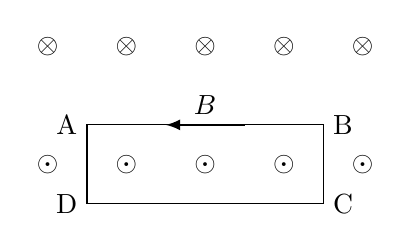
\begin{tikzpicture}
        \foreach \x in {0,...,4} {
            \node at (\x, 0) {$\odot$};
            \node at (\x, 1.5) {$\otimes$};
        }
        \draw (0.5,-0.5) -- (0.5,0.5) node[left] {A} -- (3.5,0.5) node[right] {B} -- (3.5,-0.5) node[right] {C} -- (0.5,-0.5) node[left] {D} --cycle;
        \draw[thick, -latex] (2.5,0.5) -- node[above] {$B$} (1.5,0.5);
    \end{tikzpicture}
    \caption{线圈磁场截面}
\end{figure}
如图所示,确定一个固定路径,采用Ampère's circuital law进行计算。
\begin{gather*}
    \oint_{\partial S}B\cdot dl=\mu_0\int_Sj\cdot dS\\
    \underline{Bl}_{AB}+\underline{0}_{BC}+\underline{0}_{CD}+\underline{0}_{DA}=\mu_0I\cdot nl\\
    B=\mu_0nI
\end{gather*}

\subsection{洛伦兹力推导}

使用电流的微观定义计算单个载流子的受力即可。
\begin{align*}
    \vec{f}=&\frac{\vec{F}}{N}=\frac{I\vec{l}\times\vec{B}}{N}\\
    =&\frac{nqSl\vec{v}\times\vec{B}}{nSl}\\
    =&q\vec{v}\times\vec{B}
\end{align*}

\subsection{带电粒子在磁场中运动轨迹推导}

在静磁场中带电粒子的运动方程为
\begin{equation*}
    m\frac{d^2\mathbf{r}}{dt^2}=q\frac{d\mathbf{r}}{dt}\times\mathbf{B}
\end{equation*}
假设该静磁场只存在于z方向,即$\mathbf{B}=(0,0,B)$
\begin{equation*}
    m\begin{pmatrix}
     \ddot{x}\\\ddot{y}\\\ddot{z}   
    \end{pmatrix}=
    q\begin{pmatrix}
        \dot{x}\\\dot{y}\\\dot{z}
    \end{pmatrix}\times
    \begin{pmatrix}
        0\\0\\B
    \end{pmatrix}=
    qB\begin{pmatrix}
        \dot{y}\\-\dot{x}\\0
    \end{pmatrix}
\end{equation*}
其中z方向的运动方程为$m\ddot{z}=0$,即粒子在z方向做匀速直线运动。而后,使用极坐标系处理xy平面的运动,基于其转换关系
\begin{itemize}
    \item 速度:$\begin{cases}v_r=\dot{r}\\v_\phi=r\dot{\phi}\end{cases}$
    \item 加速度:$\begin{cases}a_r=\ddot{r}-r\dot{\phi}^2\\a_\phi=2\dot{r}\dot{\phi}+r\ddot{\phi}\end{cases}$
\end{itemize}
即
\begin{align*}
    \begin{cases}
        a_r=a_x\cos\phi+a_y\sin\phi
        =\frac{qB}{m}\left(v_y\cos\phi-v_x\sin\phi\right)
        =\frac{qB}{m}v_\phi\\
        a_\phi=-a_x\sin\phi+a_y\cos\phi
        =-\frac{qB}{m}\left(-v_y\sin\phi+v_x\cos\phi\right)
        =-\frac{qB}{m}v_r\\
    \end{cases}
\end{align*}
代入运动方程可得
\begin{equation*}
    \begin{cases}
        \ddot{r}-r\dot{\phi}^2=\frac{qB}{m}r\dot{\phi}\\
        2\dot{r}\dot{\phi}+r\ddot{\phi}=-\frac{qB}{m}\dot{r}
    \end{cases}
    \implies
    \begin{cases}
        \frac{\ddot{r}}{r}=\dot{\phi}\left(\frac{qB}{m}+\dot{\phi}\right)\\
        \ddot{\phi}=-\frac{\dot{r}}{r}\left(\frac{qB}{m}+2\dot{\phi}\right)
    \end{cases}
\end{equation*}
其中一式左右两边变量完全独立,因此可以拆成两个分别等于零的式子
\begin{equation*}
    \begin{cases}
        \frac{\ddot{r}}{r}=0\\
        \dot{\phi}\left(\frac{qB}{m}+\dot{\phi}\right)=0\\
        \ddot{\phi}=-\frac{\dot{r}}{r}\left(\frac{qB}{m}+2\dot{\phi}\right)
    \end{cases}
\end{equation*}
求解联立微分方程组可得
\begin{equation*}
    \begin{cases}
        \ddot{r}=0\\
        \dot{\phi}=-\frac{qB}{m}\\
        \dot{r}=0
    \end{cases}
\end{equation*}
其物理意义即为粒子在r方向上不受力、在$\phi$方向上保持恒定角速度$\frac{qB}{m}$做圆周运动。再结合z方向的匀速直线运动可知,粒子在空间上的轨迹为圆柱螺线。

\subsection{含自感直流电路的电流表达式推导}

结合自感电势和基尔霍夫定律可得
\begin{equation*}
    E-IR+V=0
\end{equation*}
即
\begin{equation*}
    \frac{dI}{dt}=\frac{E-IR}{L}
\end{equation*}
此微分方程可解
\begin{equation*}
    I=\frac{E}{R}\left(1+C\exp\left(-\frac{R}{L}t\right)\right)
\end{equation*}
在初始条件$(t,I)=(0,0)$下可知
\begin{equation*}
    I=\frac{E}{R}\left(1-\exp\left(-\frac{R}{L}t\right)\right)
\end{equation*}

\subsection{自感线圈储能公式推导}

\begin{equation*}
    U=W=qV
    =\int_0^I(Idt)\left(L\frac{dI}{dt}\right)
    =\frac12LI^2
\end{equation*}
